
\chapter{Procédures, pile et pointeur de pile}



\section{Motivation}

Il est fréquent quand on écrit un programme d'avoir à appeler plusieurs fois une même partie de programme. Par exemple, si j'écrivais un programme de calcul, j'aurais peut être plusieurs fois besoin de calculer la racine carrée d'un nombre. Avec l'architecture que nous avons introduite jusqu'à maintenant, il nous faudrait recopier intégralement le programme qui calcule la racine carrée chaque fois qu'on en a besoin. C'est problématique pour plusieurs raisons : comme on duplique un programme on construit d'une part un programme long et d'autre part, on augmente les risques d'introduire des erreurs dans le programme. Il serait préférable d'écrire une bonne foi pour toute un programme qui calcule la racine carrée et l'appeler lorsqu'on en a besoin : c'est ce qu'on appelle une routine ou procédure. 

Prenons un autre exemple, imaginons que je souhaite calculer les premiers éléments de la suite de Syracuse définie par $u_0$ et la relation de récurrence:
\begin{eqnarray*}
\forall n \in \mathbb{N}^*, u_{n+1} =
\begin{cases}
u_n/2 & \mbox{si } u_n \mbox{ est pair}\\
3u_{n+1}+1 & \mbox{ sinon}
\end{cases}
\end{eqnarray*}

Je vous propose deux algorithmes pour calculer ces termes. L'algorithme \ref{algo:syr27} n'utilise pas de procédure et nécessite donc de répéter plusieurs fois le programme calculant le prochain élément de la suite. L'algorithme \ref{algo:syr27_proc} utilise des procédures; ce programme est beaucoup plus compact et nettement moins sujet aux erreurs d'écriture du programme.

\begin{algorithm}
\caption{\AlgoName{Suite de Syracuse sans procédures} \label{algo:syr27}}
\begin{algorithmic}[1]
\Function{Syr}{$u_0$}
\State{$u_n \gets u_0$}
\If{$u_n$ \& $0\times0001$ == 0} \Comment{Est ce que le bit de poids faible est nul ? $u_n$ pair ?}
\State $u_n \gets u_n >> 1$\Comment{Division par deux}
\Else
\State $u_n \gets 3 u_n + 1$
\EndIf
\If{$u_n$ \& $0\times0001$ == 0} \Comment{Est ce que le bit de poids faible est nul ? $u_n$ pair ?}
\State $u_n \gets u_n >> 1$\Comment{Division par deux}
\Else
\State $u_n \gets 3 u_n + 1$
\EndIf
\If{$u_n$ \& $0\times0001$ == 0} \Comment{Est ce que le bit de poids faible est nul ? $u_n$ pair ?}
\State $u_n \gets u_n >> 1$\Comment{Division par deux}
\Else
\State $u_n \gets 3 u_n + 1$
\EndIf
\EndFunction
\end{algorithmic}
\end{algorithm}


\begin{algorithm}
\caption{\AlgoName{Suite de Syracuse avec des procédures} \label{algo:syr27_proc}}
\begin{algorithmic}[1]
\Function{Syr}{$u_0$}
\State{$u_n \gets u_0$}
\State{$u_n \gets fSyr(u_n)$}
\State{$u_n \gets fSyr(u_n)$}
\State{$u_n \gets fSyr(u_n)$}
\EndFunction

\Function{fSyr}{$u_n$}
\If{$u_n$ \& $0\times0001$ == 0} \Comment{Est ce que le bit de poids faible est nul ? $u_n$ pair ?}
\State \Return $u_n >> 1$\Comment{Division par deux}
\Else
\State \Return $3 u_n + 1$
\EndIf
\EndFunction
\end{algorithmic}
\end{algorithm}

Les routines n'ajoutent pas fondamentalement de nouvelles capacités de calcul à une architecture mais sont un ingrédient d'architecture qui simplifie grandement la vie des programmeurs ou utilisateurs d'architectures informatiques, en permettant de raccourcir les programmes et d'apporter plus de robustesse face aux erreurs de programmation. Introduire les routines dans notre architecture nécessite de répondre à deux questions principales :
\begin{itemize}
\item comment passer des arguments et récupérer le résultat d'une routine ? 
\item comment se dérouter de l'exécution du programme principal pour exécuter le programme de la routine et revenir ensuite, une fois la routine terminée, dans le programme principal ?
\end{itemize}

La réponse technique à ces deux questions réside dans l'introduction d'une organisation particulière de la mémoire qu'on appelle \textbf{la pile} (\emph{stack}).


\section{La pile : modification du chemin de données et nouvelles instructions}

Une pile est une structure de données, c'est à dire un agencement particulier des données en mémoire, dite LIFO (Last In First out)\footnote{Il existe d'autres structures de données en informatique définies avec ce type d'acronyme comme par exemple les files qui sont des structures FIFO (First In First Out)}. C'est comme une pile d'assiettes : quand on ajoute un élément, on l'ajoute au sommet de la pile, quand on enlève un élément, on enlève un élément au sommet de la pile. Par convention, nous considérerons que la taille de la pile augmente vers les adresses décroissantes de la mémoire. Pour savoir à quelle adresse se trouve le sommet de la pile, nous introduisons également un nouveau registre : le registre \textbf{stack pointer} (SP). Par convention, l'adresse du sommet de pile, dans le stack pointer, sera toujours une adresse libre en mémoire. Si le sommet de pile est à l'adresse $0\times0101$, le stack pointer aura pour contenu $0\times0100$. Le nouveau chemin de données considéré est illustré sur la figure \ref{fig:chemin_seq_sp}. 


\begin{figure}[htbp]
\includegraphics[width=\linewidth]{Figs/premier_chemin_seq_sp.pdf}
\caption{\label{fig:chemin_seq_sp}Nouveau chemin de données avec l'introduction du registre de pile SP ainsi que des signaux de contrôle ReadSP et SetSP.}
\end{figure}

Il nous faut introduire deux nouveaux signaux de contrôle ReadSP et SetSP (bits 17 et 18 de la sortie de la ROM du séquenceur) et définir quelques instructions pour pouvoir initialiser et modifier le contenu de ce registre :
\begin{itemize}
\item LDSPi ($0\times8000$), LDSPd ($0\times8400$)  : chargement immédiat et direct du registre SP
\item STSP ($0\times8c00$) sauvegarde du registre SP
\item INCSP ($0\times9000$) : incrément du registre SP : \texttt{SP:=SP+1} 
\item DECSP ($0\times9400$) : décrément du registre SP : \texttt{SP:=SP-1}
\end{itemize}

On va avoir besoin de sauvegarder et de charger la valeur des registres A et B depuis la pile, on se définit donc de nouvelles instructions pour manipuler la pile :
\begin{itemize}
\item PUSHA ($0\times B000$): empile le contenu du registre A : \texttt{Mem[SP] := A; SP := SP - 1}
\item POPA ($0\times B400$): dépile le sommet de pile et place son contenu dans le registre A \texttt{SP := SP + 1; A:=Mem[SP]}
\item POKEA op ($0\times B800$): sauvegarde le contenu du registre A dans la pile \texttt{Mem[SP+operande] := A}
\item PEEKA op ($0\times BC00$): récupère le registre A dans la pile.\texttt{A := Mem[SP + op]}
\end{itemize}
Les instructions PEEK et POKE ne modifient pas le pointeur de pile. Ces instructions permettent uniquement d'aller inspecter ou modifier le contenu dans la pile sans modifier le nombre d'éléments dans la pile. On introduit aussi les instructions impliquant le registre B : PUSHB ($0\times C000$), POPB ($0\times C400$), POKEB ($0\times C800$) , PEEKB ($0\times CC00$). La figure \ref{fig:stack} illustre le fonctionnement des opérations PUSH, POP, PEEK et POKE.

% inkscape -D -z --file=stack.svg --export-pdf=stack.pdf --export-latex
\begin{figure}[htbp]
%\def\svgwidth{\columnwidth}
%    \documentclass{standalone}
\standaloneconfig{border=10pt}
\usepackage[utf8]{inputenc}
\usepackage[french]{babel}
\usepackage{amsmath}
\usepackage{cases}
\usepackage{booktabs}

\begin{document}

\renewcommand{\arraystretch}{1.2}

\begin{tabular}{@{}lllll@{}}
\textbf{\underline{Instructions pour la pile}} & & & & \\
\addlinespace[1em]
\toprule
Nom & Mnémonique & Nb. d'arguments & Opération & Opcode \\
\toprule
Load SP immédiat & LDSPi & 1 & SP := operande & 0x80\\
Load SP direct & LDSPd & 1 & SP := RAM[operande] & 0x84\\
Store SP & STSP & 1 & RAM[operande] := SP & 0x8c\\
\addlinespace[1em]
Incrémente le pointeur de pile & INCSP & 0 & SP := SP + 1 & 0x90\\
Décrémente le pointeur de pile & DECCSP & 0 & SP := SP - 1 & 0x94\\
\addlinespace[1em]
Empiler A & PUSHA & 0 & RAM[SP- -] := A & 0xb0\\
Depiler A & POPA & 0 & A := RAM[++SP] & 0xb4\\
Sauvegarder A dans la pile & POKEA & 1 & RAM[SP+operande] := A& 0xb8\\
Récupérer A dans la pile & PEEKA & 1 & A := RAM[SP+operande] & 0xbc\\
\addlinespace[1em]
Empiler B & PUSHB & 0 & RAM[SP- -] := B & 0xc0\\
Depiler B & POPB & 0 & B := RAM[++SP] & 0xc4\\
Sauvegarder B dans la pile & POKEB & 1 & RAM[SP+operande] := B& 0xc8\\
Récupérer B dans la pile & PEEKB & 1 & B := RAM[SP+operande] & 0xcc\\
\end{tabular}

\end{document}

\centering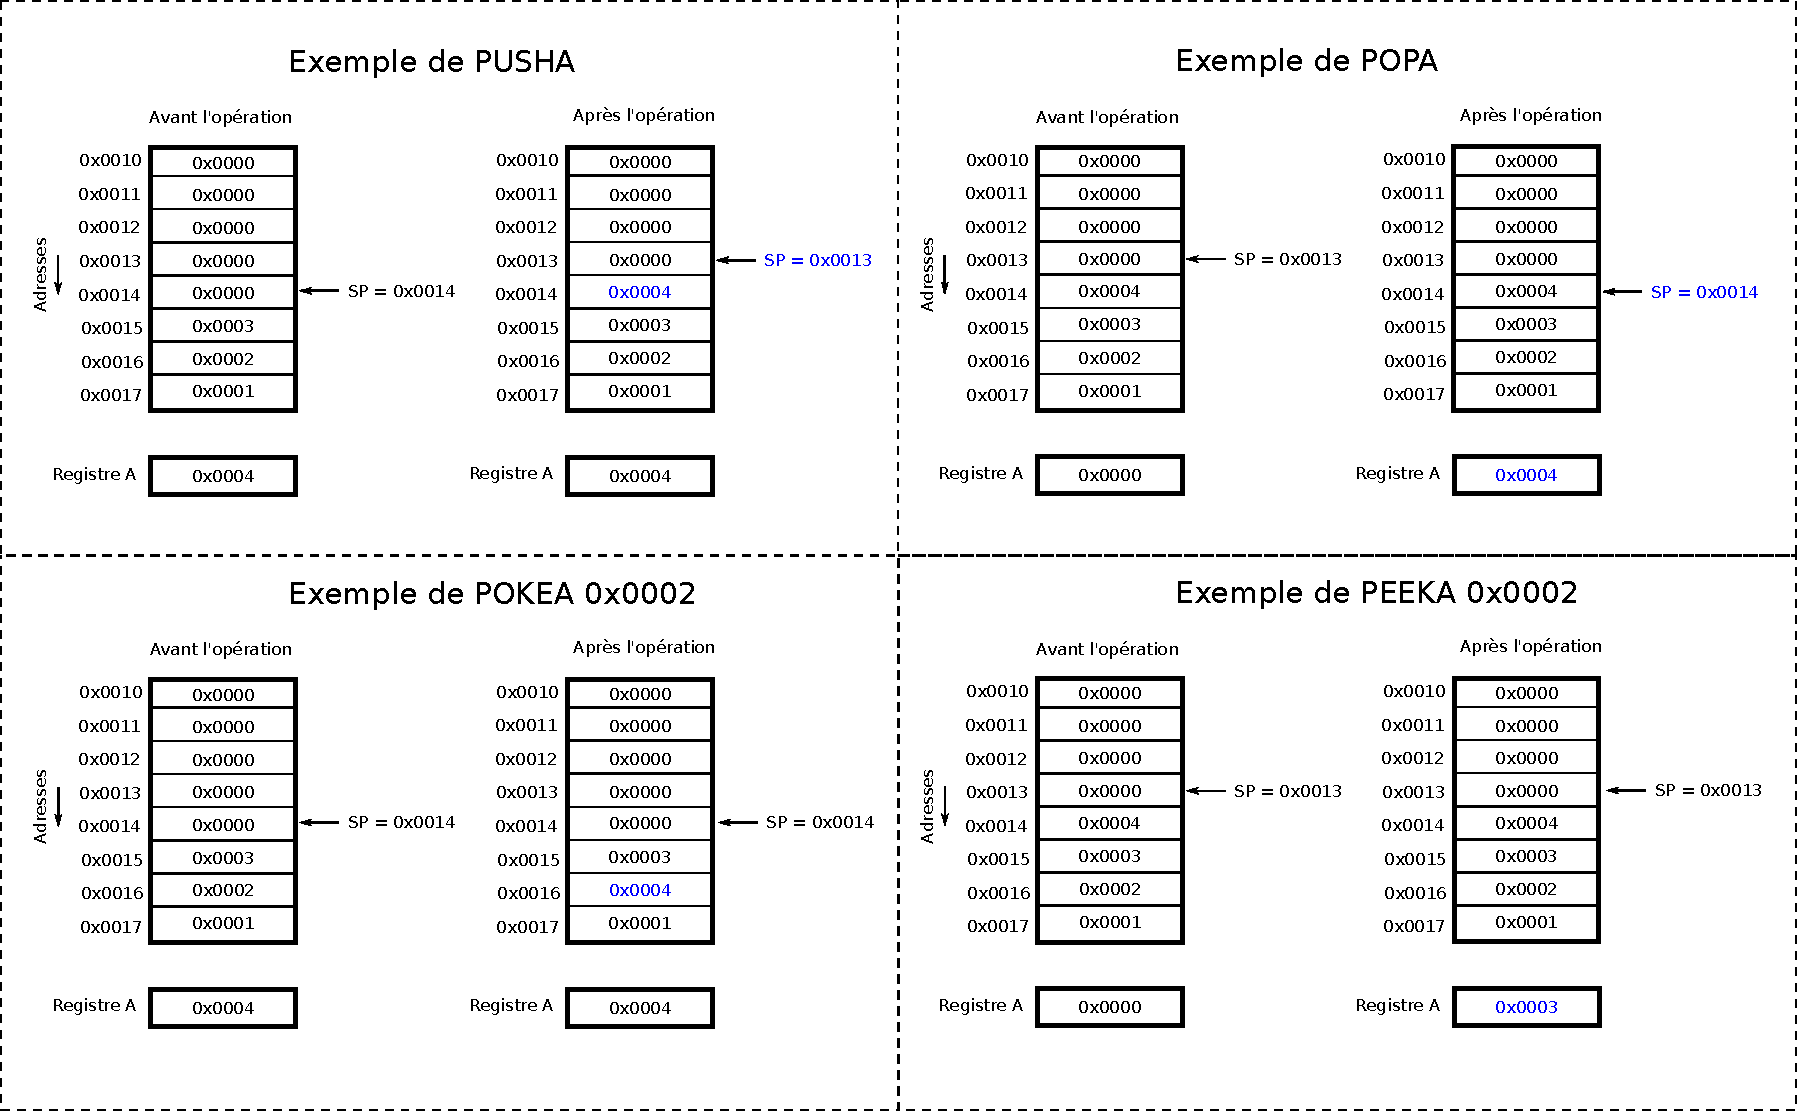
\includegraphics[width=\columnwidth]{Figs/stack.pdf}
\caption{\label{fig:stack} Le contenu de la pile est modifié par les instructions PUSH (empilement), POP (dépilement), lecture (PEEK) et modification (POKE). Les opérations PUSH et POP modifient le pointeur de pile. Par convention, l'empilement se fera toujours vers les adresses décroissantes de la mémoire.}
\end{figure}

Intéressons nous maintenant aux micro-instructions de quelques unes de nos nouvelles instructions. L'instruction PUSHA ayant le code $0\times B000$, ses micro-instructions dans la ROM commencent à l'adresse $0\times B0$ et sont:
\begin{enumerate}
\item Adresser la RAM avec le contenu du registre SP, soit ReadSP=1, UAL=0000, SetRADM=1, soit le mot hexadécimal ROM[0xB0] = $0\times00020400$
\item Transférer le contenu du registre A en mémoire, soit ReadA=1, UAL=0000, SetMem=1, soit le mot hexadécimal ROM[0xB1] = $0\times00002200$
\item décrémenter le registre de pile SP, et reboucler MicroPC à l'adresse 0x00, soit ReadSP=1, UAL=1001, SetSP=1, CodeMCount=001, @Adr=00, soit le mot hexadécimal ROM[0xB2] = $0\times00ce0000$
\end{enumerate}
Après l'exécution de l'instruction PUSHA, on a mémorisé le contenu du registre dans la pile et également décrémenter le registre SP pour garantir que le pointeur de pile soit de nouveau sur une zone libre de la mémoire. Pour l'instruction POPA, il nous faut dépiler le sommet de pile dans le registre A. Puisque le pointeur de pile pointe sur la prochaine zone libre de la mémoire, il faut incrémenter le pointeur de pile avant de lire la mémoire. L'instruction POPA ayant le code $0\times B400$, ses micro-instructions dans la ROM commencent à l'adresse $0\times B4$ et sont :
\begin{enumerate}
\item incrémenter le pointeur de pile et le stocker dans SP et RADM, soit ReadSP=1, UAL=1000, SetSP=1, SetRADM=1, soit le mot hexadécimal ROM[0xB4] = $0\times00460400$
\item lire la mémoire et transférer son contenu dans le registre A et également reboucler MicroPC à l'adresse 0x00, soit ReadMem=1, UAL=0001, SetA=1, CodeMCount=001, @Adr=00, soit le mot hexadécimal ROM[0xB5] = $0\times00884100$
\end{enumerate}

Les instructions POKE et PEEK prennent une opérande. Elles permettent de modifier ou lire le contenu d'un élément de la pile, en y faisant référence grâce à l'opérande. Par exemple, l'instruction PEEKA 0x0002 charge dans le registre A le contenu de la pile à l'adresse SP+0x0002 et l'instruction POKEA 0x0002 sauvegarde le contenu du registre A dans la pile à l'adresse $SP + 0\times0002$. L'instruction POKEA ayant le code $0\times B800$, ses micro-instructions dans la ROM commencent à l'adresse $0\times B8$ et sont~:
\begin{enumerate}
\item adresser la RAM avec le contenu de PC, soit ReadPC=1, UAL=0000, SetRadm=1, soit le mot hexadécimal ROM[0xB8] = $0\times00000c00$
\item additionner le contenu de la mémoire et du registre SP et stocker le résultat dans RADM, soit ReadMem=1, ReadSP=1, UAL=0110, SetRADM=1, soit le mot hexadécimal ROM[0xB9] = $0\times00320500$
\item sauvegarder le contenu du registre A en mémoire, soit ReadA=1, UAL=0000, SetMem=1, soit le mot hexadécimal ROM[0xBA] = $0\times00002200$
\item incrémenter le PC et reboucler MicroPC à l'adresse 00, soit ReadPC=1, UAL=1000, SetPC=1, CodeMCount=001, @Adr=00, soit le mot hexadécimal ROM[0xBB] = $0\times00c01800$
\end{enumerate}
L'instruction PEEKA ayant le code $0\times BC00$, ses micro-instructions dans la ROM commencent à l'adresse $0\times BC$ et sont~:
\begin{enumerate}
\item adresser la RAM avec le contenu de PC, soit ReadPC=1, UAL=0000, SetRadm=1, soit le mot hexadécimal ROM[0xBC] = $0\times00000c00$
\item additionner le contenu de la mémoire et du registre SP et stocker le résultat dans RADM, soit ReadMem=1, ReadSP=1, UAL=0110, SetRADM=1, soit le mot hexadécimal ROM[0xBD] = $0\times00320500$
\item charger le contenu de la mémoire dans le registre A, soit ReadMem=1, UAL=0001, SetA=1, soit le mot hexadécimal ROM[0xBE] = $0\times00084100$
\item incrémenter le PC et reboucler MicroPC à l'adresse 00, soit ReadPC=1, UAL=1000, SetPC=1, CodeMCount=001, @Adr=00, soit le mot hexadécimal ROM[0xBF] = $0\times00c01800$
\end{enumerate}





\section{La pile pour passer des arguments et récupérer des résultats}

La procédure introduite précédemment \texttt{fsyr} nécessite un argument et retourne un résultat. Ce ne serait pas une bonne idée d'utiliser que les registres pour stocker les opérandes et les résultats parce qu'on s'interdirait des routines qui appelle des routines qui appelle des routines, etc.. (comme les fonctions récursives comme la factorielle dont nous reparlerons). La bonne structure pour passer des arguments et récupérer des résultats est \textbf{une pile}. La pile est la structure de données appropriée pour passer des arguments à une routine, stocker des éventuelles variables locales dont on pourrait avoir besoin dans la routine, et stocker l'éventuel résultat de la routine que le programme appelant pourra récupérer. Considérons par exemple une routine qui calcule la somme des entiers de $0$ à $N$ inclus, appelée depuis un certain programme principal, et donnée par l'algorithme \ref{algo:sum_N}.

\begin{algorithm}
\caption{\AlgoName{Somme des entiers de $0$ à $N$} \label{algo:sum_N}}
\begin{algorithmic}[1]
\Function{somme}{$N$}
\State{Soient $i$, $res$ deux variables locales}
\For{$i$ de $0$ à $N$}
\State{$res \gets res + i$}
\EndFor
\State \Return $res$
\EndFunction

\Function{main}{}
\State somme($3$)
\EndFunction
\end{algorithmic}
\end{algorithm}


L'idée d'utiliser la pile pour stocker les arguments de la routine est que le programme principal les empile avant d'exécuter le programme de la routine. On verra dans la prochaine section comment exécuter la routine, pour le moment, on se concentre sur les arguments, les variables locales et le résultat. Donc, l'appel de routine va se passer de la manière suivante :
\begin{enumerate}
\item le programme principal réserve de la place sur la pile, en décrémentant le pointeur de pile pour pouvoir mémoriser le résultat de la routine
\item le programme principal empile l'argument de la routine, dans notre exemple la valeur 3
\item la machine part pour l'exécution de la routine 
\item le programme de la routine récupère l'argument de la pile (sans le dépiler)
\item le programme de la routine s'exécute en mémorisant sur la pile les éventuelles variables locales (comme $i$ et $res$ dans notre exemple)
\item à la fin du programme de la routine, les variables locales sont dépilées et la routine sauvegarde son résultat dans l'espace réservé par le programme principal
\item de retour au programme principal, on dépile le ou les arguments et on dépile le résultat
\end{enumerate}

\begin{figure}[htbp]
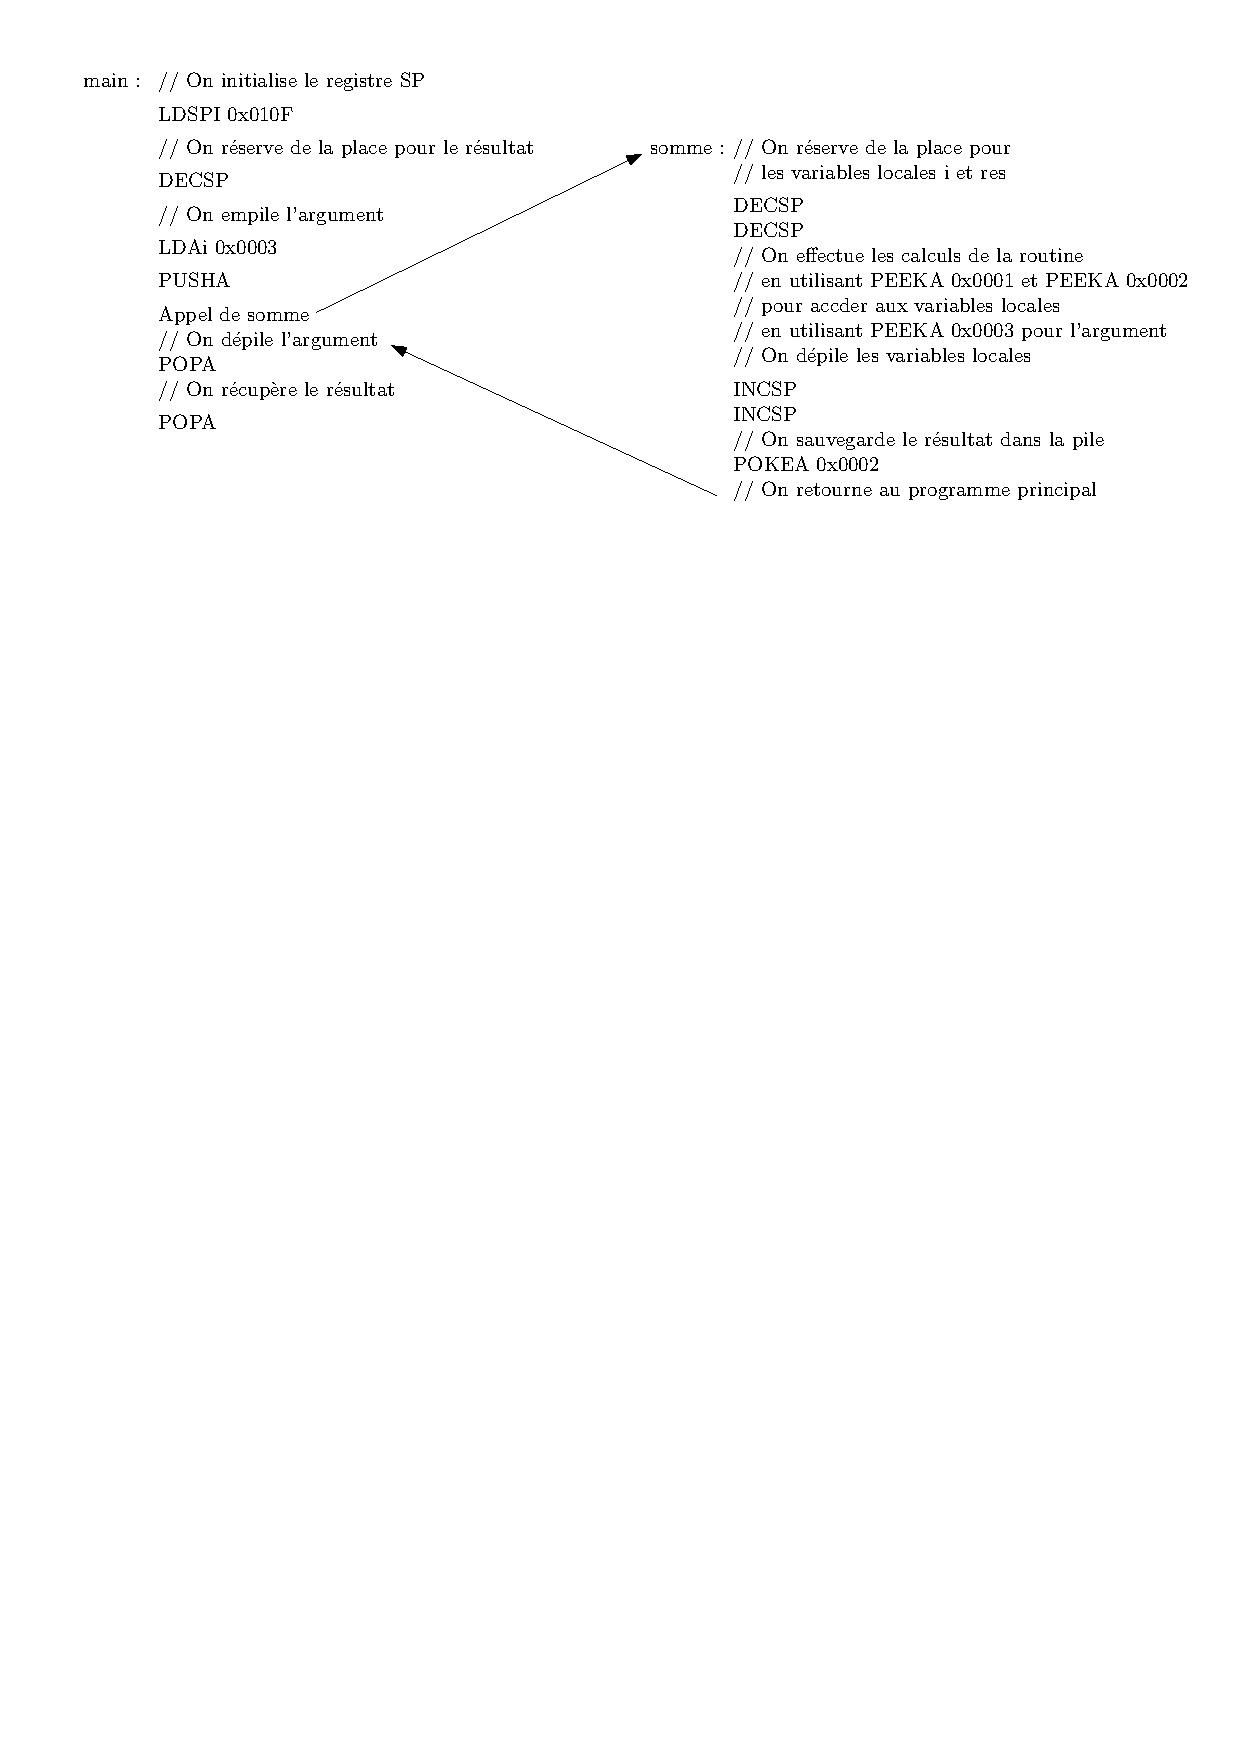
\includegraphics[width=.9\columnwidth]{Figs/stack_args.pdf}
\caption{\label{fig:stack_args} Représentation schématique montrant l'appel d'une routine avec le passage d'arguments et la sauvegarde du résultat.}
\end{figure}


Ce déroulement est représenté schématiquement sur la figure \ref{fig:stack_args}. L'important est de s'assurer qu'il y a toujours autant d'éléments dans la pile quand on part vers l'exécution de la routine et quand on en revient. C'est bien donc la responsabilité du programme appelé que de supprimer les éventuelles variables locales allouées sur la pile et la responsabilité du programme appelant de faire le ménage sur la pile pour l'argument et le résultat. Les variables locales sont, dans cette version de l'architecture, accessible par rapport à la valeur courante du pointeur de pile. Les variables $res$ et $i$ sont aux adresses $SP + 0\times0001$ et $SP+ 0\times0002$. Notez que ça peut devenir compliqué de savoir à quelle adresse se trouve les arguments puisqu'il faut prendre en compte le nombre de variables locales allouées. Une autre façon de faire consiste à introduire un nouveau registre, le \emph{base pointer}. Dans notre cas, après avoir réservé de la place pour les variables locales, l'argument est à l'adresse $SP + 0\times0003$.

Imaginons que le registre SP (stack pointer) soit initialisé à la valeur $0\times010F$, la figure \ref{fig:stack_args_fig} illustre alors l'évolution de la pile et des registres autour de l'appel de la routine. 

\begin{figure}[htbp]
\includegraphics[width=\columnwidth]{Figs/stack_args_fig.pdf}
\caption{\label{fig:stack_args_fig} Illustration du contenu de la pile après quelques unes des instructions du programme illustré sur la figure \ref{fig:stack_args}.}
\end{figure}



\section{Appel et retour de routines}

Il nous reste maintenant à voir comment faire pour que la machine soit déroutée du programme principal vers le programme de la routine pour ensuite revenir au programme principal. Fondamentalement, le problème revient à savoir mettre les bonnes valeurs dans le registre PC qui, je vous le rappelle, pointe dans la mémoire le programme à exécuter. Le départ en routine n'est rien d'autre qu'un branchement à l'adresse à laquelle se trouve la première instruction de la routine. Si le programme de la routine se trouvait à l'adresse $0\times0020$ en mémoire, il suffit d'appeler l'instruction JMP 0x0020 pour appeler la routine somme. Le principal problème concerne en fait le retour de routine. La routine pouvant être appelée plusieurs fois dans le programme principal, comment savoir à quelle adresse retourner après avoir fini d'exécuter la routine ? La réponse est qu'il suffit de sauvegarder sur la pile la valeur du registre PC juste avant de partir exécuter la routine. Attention, il faut sauvegarder la valeur du registre PC après avoir lu l'adresse de la routine et on introduit pour le coup deux nouvelles instructions : CALL ($0\times A000$) et RET  ($0\times A800$) définies comme suit :
\begin{itemize}
\item CALL op : départ vers une routine en chargeant dans le registre PC la valeur de op et en empilant la valeur du PC \textbf{après} avoir lu l'opérande, ce qu'on appelle \textbf{l'adresse de retour}
\item RET : retour de routine en dépilant l'adresse de retour de la pile
\end{itemize}

Puisque la routine peut avoir besoin d'utiliser les registres A et B, on va introduire \textbf{la convention que c'est au programme appelant de sauvegarder sur la pile le contenu des registres A et B} (avec des PUSHA, PUSHB) si il les utilisent \textbf{et de les dépiler} (POPA, POPB) après être revenu de la routine. On dit alors que les registres A et B sont \emph{caller-save}. 


Il faut également faire attention à l'adresse de retour qui est sauvegardée dans la pile. L'adresse de retour à sauvegarder est en effet l'adresse mémoire du mot qui suit l'opérande de l'instruction CALL. C'est à dire que lorsque le PC pointe sur l'opérande de CALL, il faut sauvegarder PC+1 dans la pile.

L'instruction CALL ayant pour code $0\times A0$, ses micro-instructions commencent dans la ROM à l'adresse $0\times A0$ et sont :
\begin{enumerate}
\item on adresse la mémoire avec le contenu de SP, soit ReadSP=1, UAL=0000, SetRadm=1,% 00020400
\item on calcule l'adresse de retour et on la sauvegarde dans la pile, soit ReadPC=1, UAL=1000, SetMem=1 % 00400a00
\item on décrémente le pointeur de pile, soit ReadSP=1, UAL=1001, SetSP=1, % 004e0000
\item on adresse la mémoire avec le contenu de PC pour accéder à l'opérande du CALL, soit ReadPC=1, UAL=0000, SetRadm=1 %00000c00
\item on charge le PC avec l'adresse de la routine en mémoire et on reboucle MicroPC à l'adresse 0x00, soit ReadMem=1, UAL=0001, SetPC=1, CodeMCount=001, @Adr=00,% 00881100
\end{enumerate}

%% Par ailleurs, la mise en oeuvre des micro-instructions de l'instruction CALL pose un petit soucis technique. L'adresse de retour qui doit être sauvegardée dans la pile lorsque l'instruction CALL est invoquée est la valeur du PC \textbf{après} avoir lu l'opérande du CALL. Dans le cas de notre architecture, on peut envisager deux solutions. L'une d'elle consiste à calculer et sauvegarder l'adresse PC+1 lorsque le PC pointe sur l'opérande du CALL. Une deuxième solution, qui est celle que nous allons mettre en oeuvre, consiste à stocker dans un registre temporaire l'opérande du CALL puis à incrémenter le PC et à sauvegarder cette valeur dans la pile. Pour ce faire, nous introduisons le registre temporaire Temp et ses signaux de contrôle SetT, ReadT comme sur la figure \ref{fig:chemin_seq_sp_tmp}.



%% \begin{figure}[htbp]
%% \includegraphics[width=\linewidth]{Figs/premier_chemin_seq_sp_tmp.pdf}
%% \caption{\label{fig:chemin_seq_sp_tmp} Nouveau chemin de données avec l'introduction du registre temporaire Temp ainsi que des signaux de contrôle ReadT et SetT.}
%% \end{figure}

%% L'instruction CALL ayant pour code $0\times A0$, ses micro-instructions commencent dans la ROM à l'adresse $0\times A0$ et sont :
%% \begin{enumerate}
%% \item on adresse la mémoire avec le contenu de PC pour accéder à l'opérande du CALL, soit ReadPC=1, UAL=0000, SetRadm=1 %00000c00
%% \item on lit l'adresse de la routine en mémoire et on la sauvegarde dans le registre Temp, soit ReadMem=1, UAL=0001, SetT=1 % 00084100
%% \item on adresse la mémoire avec le contenu de SP pour empiler l'adresse de retour, soit ReadSP=1, UAL=0000, SetRadm=1 % 00020400
%% \item on calcule l'adresse de retour et on la sauvegarde dans la pile, soit ReadPC=1, UAL=1000, SetMem=1 % 00400a00
%% \item on décrémente le pointeur de pile, soit ReadSP=1, UAL=1001, SetSP=1, % 004e0000
%% \item on charge le PC avec le contenu du registre Temp et on reboucle MicroPC à l'adresse 0x00, soit ReadT=1, UAL=0001, SetPC=1, CodeMCount=001, @Adr=00, % 00803000
%% \end{enumerate}

L'instruction RET ayant pour code $0\times A800$, ses micro-instructions commencent dans la ROM à l'adresse $0\times A8$ et sont~:
\begin{enumerate}
\item on incrémente le registre SP et on sauvegarde le résultat dans SP et RADM (pour accéder à l'adresse de retour), soit ReadSP=1, UAL=1000, SetSP=1, SetRADM=1, %00460400
\item on transfert l'adresse retour en mémoire vers le PC et on reboucle MicroPC à l'adresse 0x00, soit ReadMem=1, UAL=0001, SetPC=1, CodeMCount=001, @Adr=00, %00881100
\end{enumerate}

Sur la figure \ref{fig:respo_pile}, je vous propose un résumé de nos conventions d'utilisation de la pile. 

\begin{figure}[htbp]
\centering\includegraphics[width=\linewidth]{Figs/respo_pile.pdf}
\caption{\label{fig:respo_pile} Résumé des responsabilités d'allocation et de désallocation d'espace sur la pile.}
\end{figure}

Lorsqu'une routine doit être appelée, c'est la responsabilité de l'appelant que de sauvegarder éventuellement les registres A et B (caller-save), d'allouer de la place pour le résultat de la routine et d'empiler les arguments. L'instruction CALL qui vient ensuite se charge d'empiler l'adresse de retour. La routine peut empiler d'autres valeurs, comme des variables locales, sur la pile. Lorsque la routine se termine, celle-ci doit remettre le pointeur de pile à l'état dans lequel elle l'a trouvé à son appel. Les architectures actuelles utilisent pour cela des registres particuliers \emph{base pointer} et \emph{frame pointer} pour restaurer en un coup d'horloge le pointeur de pile sans que le programme de la routine n'ait à dépiler explicitement des éléments de la pile. Ces registres permettent également d'adresser facilement les variables par rapport à une base de la pile fixe plutôt que relativement à une tête flottante. Pour l'architecture que nous étudions ici, on se limitera à l'utilisation du seul registre \emph{stack pointer}. On dit que le registre de pile SP est \emph{callee-save} : le programme appelant a la garantie d'avoir dans le registre SP la même valeur avant et après l'appel de routine. L'instruction RET récupère alors l'adresse de retour et c'est le programme appelant qui a en charge de dépiler les arguments, le résultat et les sauvegardes éventuelles des registres.



Pour illustrer le comportement de l'architecture lors de l'appel et du retour de routines, je vous propose de considérer un programme qui appelle une routine $f(a,b) = a+b$. La représentation en mémoire de ce programme et la routine en utilisant les noms des instructions pour plus de lisibilité est donnée ci-dessous~:

\begin{verbatim}
# Programme appelant :
0x0000     LDSPi 0x0030
0x0002     DECSP          # On réserve de la place dans la pile pour la valeur de retour
0x0003     LDAi  0x0007
0x0005     PUSHA          # On charge la première opérande
0x0006     LDAi  0x0008
0x0008     PUSHA          # On charge la deuxième opérande
0x0009     CALL 0x0020    # On appelle la routine
0x000b     POPA           # On enlève la deuxième opérande de la pile
0x000c     POPA           # On enlève la première opérande de la pile
0x000d     POPA           # On récupère le résultat
0x000e     STA  0x1000    # On affiche le résultat
0x0010     END            # Fin de programme

# Routine à l'adresse 0x0020:
0x0020     PEEKA 0x0003   # On récupère la première opérande
0x0022     PEEKB 0x0002   # On récupère la seconde opérande
0x0024     ADDA           # On en fait la somme
0x0025     POKEA 0x0004   # On sauvegarde le résultat
0x0027     RET            # On retourne au programme appelant
\end{verbatim}

L'évolution de la pile pendant l'exécution ce programme est donnée sur la figure \ref{fig:stack_ab}. La seule nouveauté ici est de remarquer ce qui se passe aux appels de CALL et RET. Lors du CALL, l'adresse de retour $0\times000b$ est empilée et le registre PC est chargé avec la valeur $0\times0020$ pour exécuter le programme de la routine. Lors du RET, l'adresse de retour $0\times000b$ est dépilée et chargée dans le registre PC. Le programme ci-dessus est écrit en utilisant le nom des instructions; pour pouvoir être utilisé sur l'architecture, il suffit de traduire chacune des instructions avec son code comme sur la figure\ref{fig:traduction_asm_machine}. Un programme écrit avec les noms des instructions est un programme écrit en langage d'assemblage et sa traduction automatique en code machine est l'objet du prochain chapitre.

\begin{figure}[htbp]
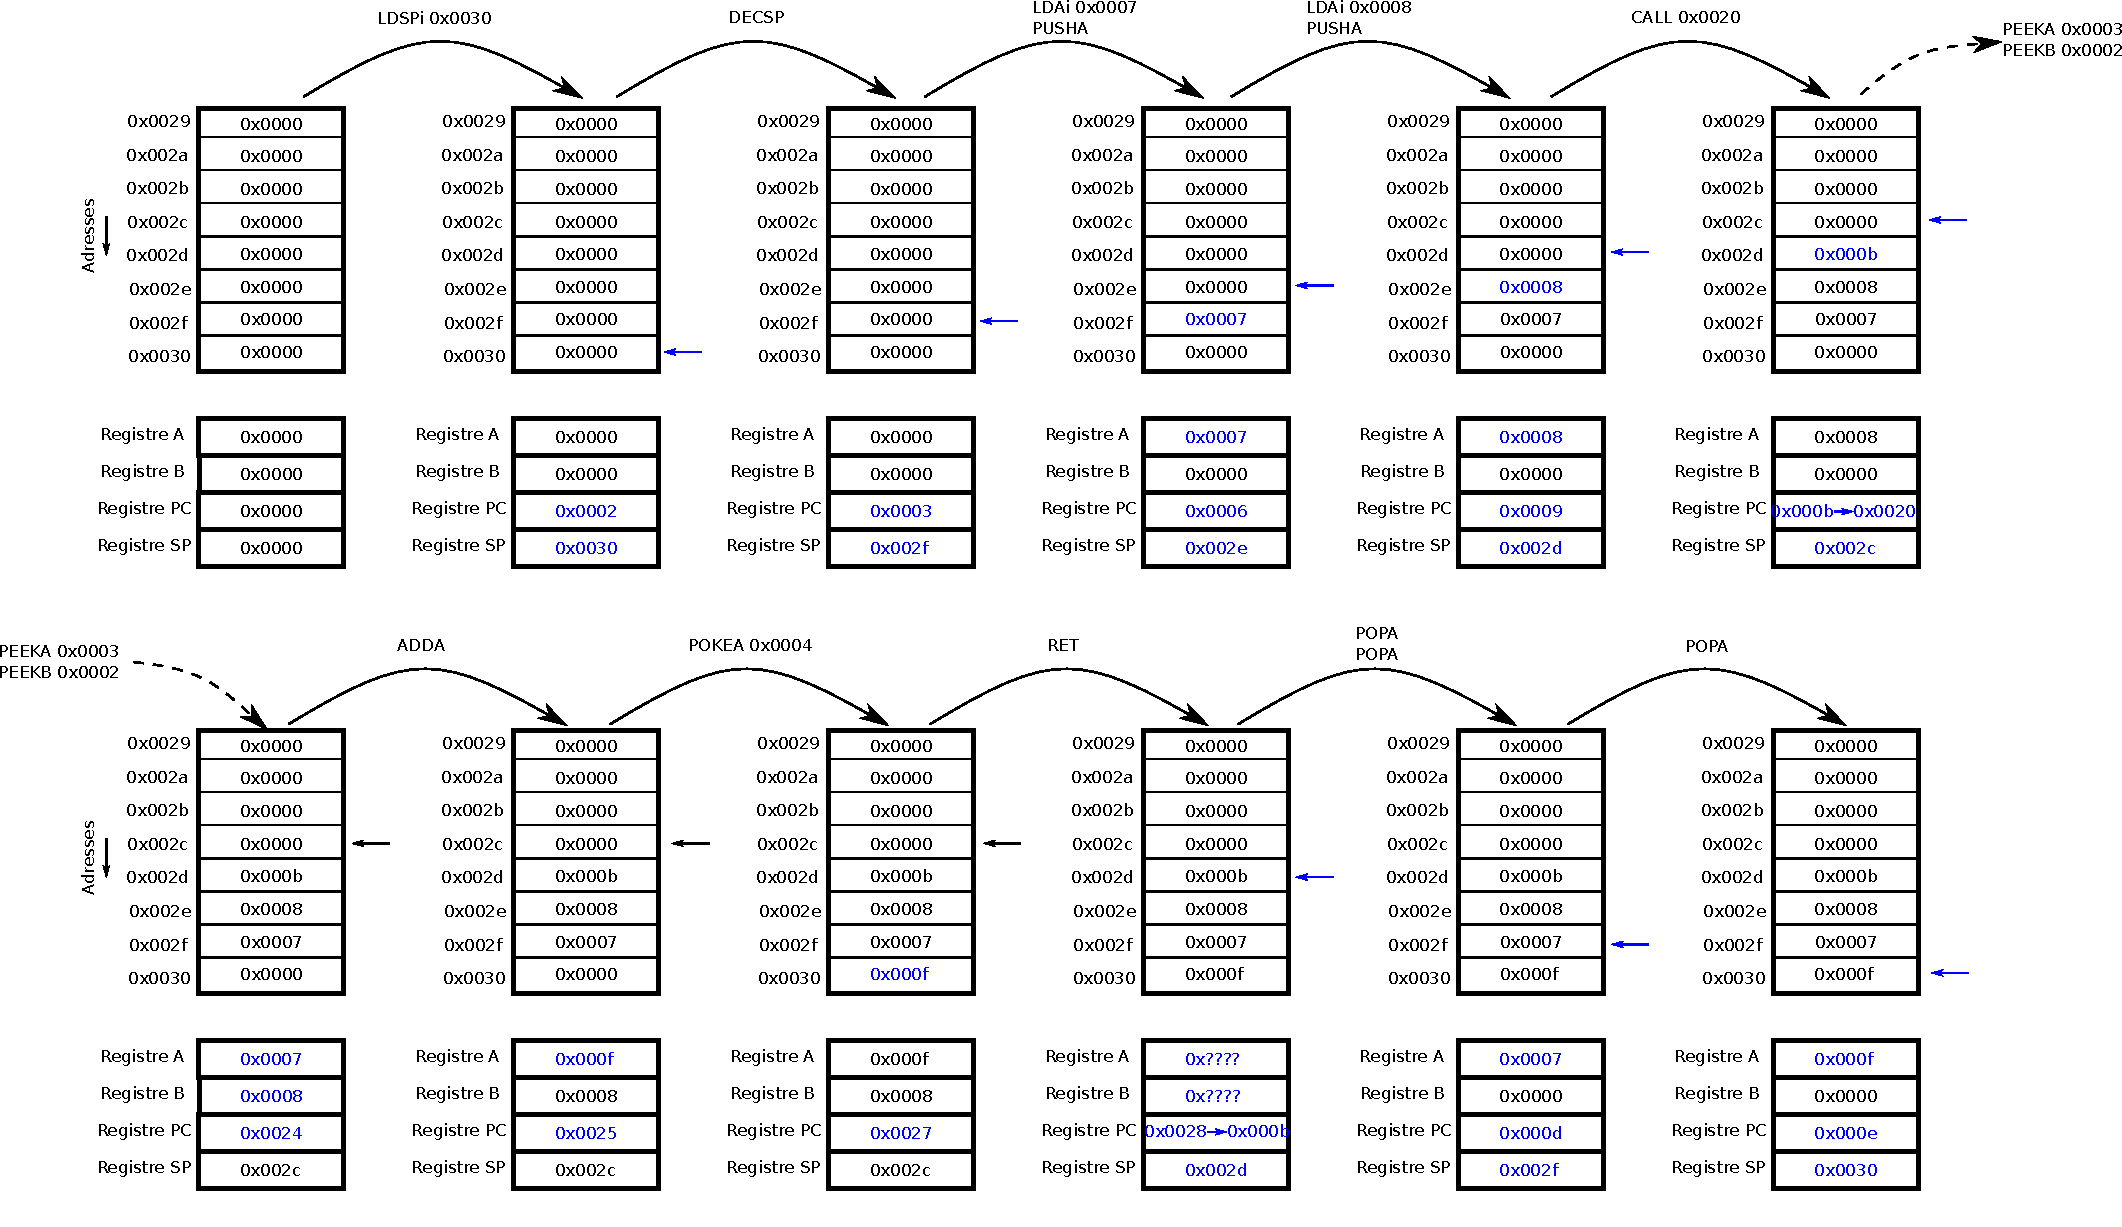
\includegraphics[width=\linewidth]{Figs/stack_call_ret.pdf}
\caption{\label{fig:stack_ab} Illustration de la pile pendant l'exécution d'un programme qui appelle une routine calculant $f(a,b) = a+b$. Notez qu'aucune garantie n'est donnée sur les valeurs des registres A et B après l'appel de la routine. C'est donc à la responsabilité de l'appelant de sauvegarder le contenu de ces registres si il les utilise.}
\end{figure}

\begin{figure}[htbp]
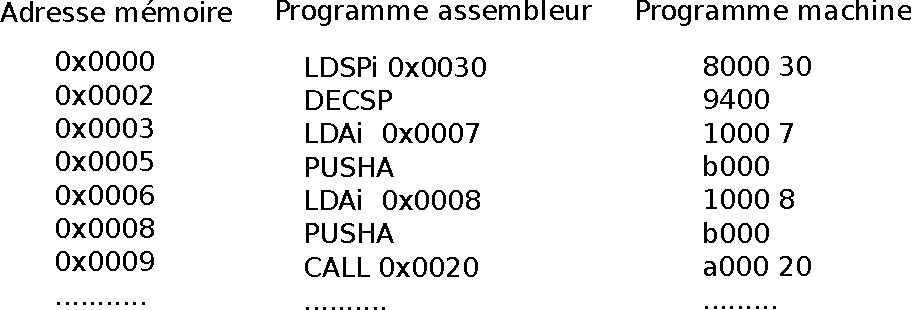
\includegraphics[width=0.7\linewidth]{Figs/traduction_asm_machine.pdf}
\caption{\label{fig:traduction_asm_machine} Un programme écrit en langage d'assemblage, i.e., utilisant le nom des instructions, peut se traduire directement en code binaire en utilisant le code de chacune des instructions.}
\end{figure}


\section{Exemple : nombre de mouvements pour résoudre les tours de Hanoï}

Les tours de Hanoï est un jeu construit à partir de trois piliers et $n$ palets de taille différente. Le jeu débute avec tout les palets empilés sur le pilier le plus à gauche par ordre de taille décroissante, le but étant de déplacer tout les palets vers le pilier le plus à droite, comme illustré sur la figure \ref{fig:hanoi}. Les déplacements des palets sont contraints par quelques règles :
\begin{itemize}
\item on ne déplace pas plus d'un palet à la fois,
\item chaque mouvement consiste à déplacer le premier palet d'un pilier vers un autre pilier
\item un palet ne peut pas être déposé sur un palet plus petit
\end{itemize}

\begin{figure}[htbp]
\includegraphics[width=\linewidth]{Figs/hanoi.pdf}
\caption{\label{fig:hanoi} Configuration initiale et cible du problème des tours de Hanoi.}
\end{figure}

On s'intéresse ici à calculer le nombre de déplacement minimum nécessaire pour résoudre un puzzle à $n$ palets. Soit $h(n)$ le nombre minimum de mouvements nécessaires pour déplacer $n$ palets. Si $n=1$, il suffit d'un mouvement. Pour résoudre le problème à $n$ palets, $n > 1$, il suffit de déplacer les $n-1$ premiers palets du premier pilier au second, puis de déplacer le dernier palet sur le dernier pilier et enfin de déplacer les $n-1$ palets du pilier du milieu sur le dernier pilier, de telle sorte que $h(n)$ est définie par la récurrence :
\begin{eqnarray*}
h(n) = \begin{cases}
1 & \mbox{si } n=1 \\
2h(n-1) + 1 & \mbox{sinon}
\end{cases}
\end{eqnarray*}
La valeur de $h(n)$ faisant intervenir $h(n-1)$, on parle de fonction récursive. Le cas $n=1$ est appelé cas terminal\footnote{quand on construit une fonction récursive, il faut toujours s'assurer que la récursion nous rapproche d'un cas terminal, sans quoi il est impossible de calculer sa valeur}. Je vous propose de construire un programme pour notre architecture qui calcule, disons, $h(4)$. Pour ce faire, nous construisons un programme principal qui fait appel à une routine qui calcule $h(n)$.
\begin{verbatim}
# Programme principal :
0x0000     LDSPi 0x0FFF
0x0002     DECSP          # On réserve de la place dans la pile pour la valeur de retour
0x0003     LDAi  0x0004
0x0005     PUSHA          # On charge l'opérande
0x0006     CALL 0x000D    # On appelle la routine
0x0008     POPA           # On enlève l'opérande
0x0009     POPA           # On récupère le résultat dans A
0x000A     STA  0x1000    # On l'affiche
0x000C     END
#routine
0x000D     PEEKA 0x0002   # On récupère n qui se trouve à l'adresse SP+0x0002
                          # puisque SP+0x0001 contient l'adresse de retour
0x000F     LDBi 0x0001
0x0011     SUBB           # On calcule B:= n - 1
0x0012     JZB  0x0023    # Si B = 0, i.e. n=1, on branche en 0x0023
                          # Sinon on invoque h(n-1)
0x0014     DESCP          # On réserve de la place pour la valeur de retour
0x0015     PUSHB          # On empile l'opérande n-1
0x0016     CALL 0x000D    # On appelle la routine h(n-1)
0x0018     INCSP          # On enlève l'opérande
0x0019     POPA           # On récupère le résultat h(n-1) dans A
0x001A     LDBi 0x0002    
0x001C     MULA           # On calcule A := 2*h(n-1)
0x001D     LDBi 0x0001   
0x001F     ADDA           # On calcule A:= 2*h(n-1) + 1
0x0020     POKEA 0x0003   # On sauvegarde le résultat  dans la pile
0x0022     RET            # On retourne à l'appelant
0x0023     LDAi  0x0001
0x0025     POKEA 0x0003   # On sauvegarde le résultat terminal h(1) = 1
0x0027     RET
\end{verbatim}
 
L'évolution de la pile pendant l'exécution de ce programme est représentée sur la figure \ref{fig:hanoi_stack}.
\begin{figure}[htbp]
\includegraphics[width=\linewidth]{Figs/hanoi_stack.pdf}
\caption{\label{fig:hanoi_stack} Evolution de la pile pendant les appels de routine. La réservation de la place pour le résultat le placement des opérandes est faite avant les instructions CALL. L'adresse de retour est placée sur la pile par l'instruction CALL.}
\end{figure}

Les fonctions récursives non terminales ont ce comportement particulier de pile qui croît au fur et à mesure des appels et décroît au fur et à mesure de la construction des résultats. Que se passe t'il si on ne définit pas de cas terminal ou si les appels récursifs n'atteignent pas le cas terminal (un bug fréquent) ? Les architectures sont conçues de telle sorte que la pile ne puisse pas dépasser une certaine taille et le programme retournera alors ``stack overflow'', i.e. un débordement de pile.

%% \pagebreak
%% \newpage
%% \section{Récapitulons}

%% comme dans le chapitre ISA mais en ajoutant les nouvelles instructions.



%% \pagebreak
%% \newpage
%% \section{Compléments}



%% \subsection{Le base pointer pour faciliter l'adressage de la pile}
%% \label{sec:base_pointer}
%% \subsection{Le frame pointer pour faciliter le ``nettoyage'' de la pile}
%% \subsection{Le link register pour accélérer le retour de procédures}
%% \subsection{Conventions de sauvegarde des registres : caller-saved et callee-saved}

%% \subsection{Notes}


%% Callee save convention : c'est la procédure appelée qui sauvegarde les registres qu'elle utilise de telle sorte que l'appelant retrouve ses registres dans l'état qu'il les avait laissé;

%% Link Register : le caller met dedans l'adresse de retour

%% Base pointer : plus facile pour accéder aux variables locales

%% il empile arg n-1, arg n-2 , ... arg 0 ; en indiquant que c'est super important si jamais il y a des side effects ?!?!?! On peut en fait facilement gérer un nombre variable d'argument. En utilisant le BP, le premier argument est toujours au même offset par rapport à BP. L11 38 min : convention caller/callee


%% plus tard il parle de cloture : mécanisme qui permet à des procédures de retourner des procédures qui capturent des variables.
